\centerline{\bf \Huge Признаки равенства треугольников}

\begin{flushright}
        \scriptsize{Авраам Линкольн дал людям свободу, \\
                    а полковник Кольт уравнял их шансы}
\end{flushright}

\textbf{\Large{Первый признак равенства.}}

\problem{1}
Все стороны и углы пятиугольника равны. Докажите, что равны и все диагонали.

\problem{2}
Два квадрата имеют общую вершину. Докажите, что отмеченные пунктиром на рисунке отрезки равны (по определению у квадрата все стороны равны, а углы прямые).

\begin{center}
    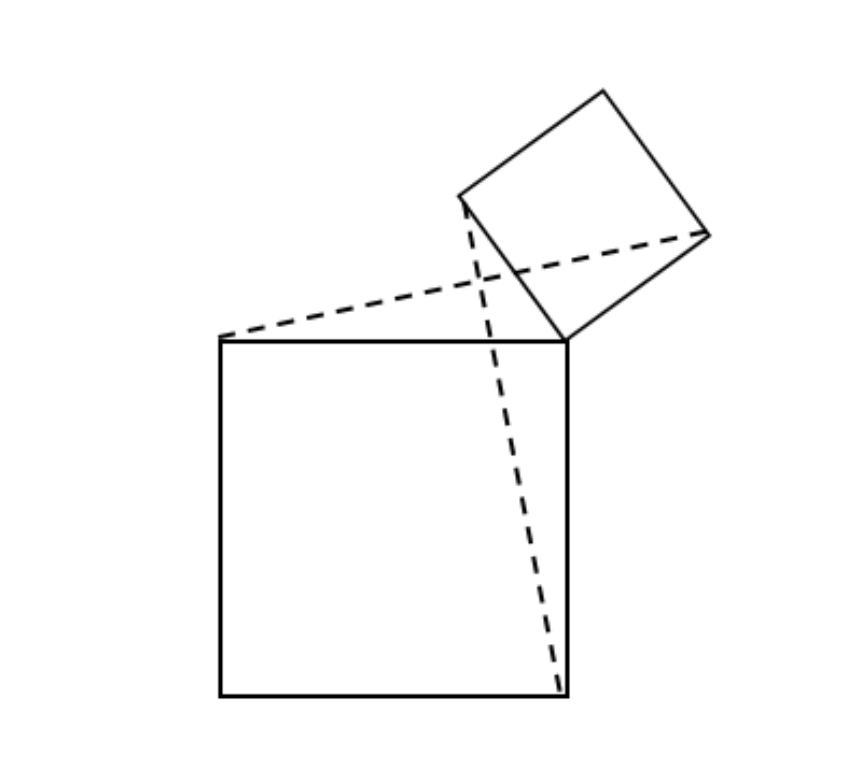
\includegraphics[width=0.4\textwidth]{Сборы/Сборы Элиста 2025/РВ/8/Признаки равенства/Условия/1.3.png}
\end{center}

\textbf{\Large{Второй признак равенства.}}

\problem{3}
Дан угол $A O B$ и точка $K$ на его биссектрисе. Докажите, что перпендикуляры, опущенные из точки $K$ на стороны угла, равны. Говорят, что тогда точка $К$ «равноудалена от сторон угла».

\problem{4}
Дан четырехугольник $A B C D$, в котором $\angle B A C=\angle B D C, \angle C A D=\angle A D B$. Докажите, что $A B=C D$.

\textbf{\Large{Третий признак равенства.}}

\problem{5}
Дан четырехугольник $A B C D$, у которого $A B=A D, B C=C D$. На диагонали $A C$ отмечена точка $K$. Докажите, что $B K=K D$.

\problem{6}
Противоположные стороны четырехугольника равны. Докажите, что его диагонали делятся точкой пересечения пополам.